%! TEX root = ../main.tex

\chapter{Monte Carlo simulations and probability density functions}%
\label{apdx:magepdfs}

\blocktitle{MaGe}
Background components that were identified in the energy spectra or in radio-purity
screening measurements (see \cref{apdx:assay}) are simulated using the \mage\
software~\cite{Boswell2011} based on \geant~\cite{Agostinelli2002, Allison2006,
Allison2016}.  The \gerda\ \phasetwo\ detectors, their arrangement in seven strings as
well as the LAr instrumentation are implemented into \mage. A graphic rendering of the
relevant implemented hardware components is presented in~\cref{fig:setup:magevolumes}.
\newpar
Simulations of radioactive decays and full tracking of the decay products are performed in
all the hardware components close enough to the detector. Relevant event data like energy
depositions in sensitive detectors (germanium, LAr, SiPMs and PMTs), hit location in
germanium and LAr is written on disk. Propagation of optical photons (e.g.~resulting from
the LAr scintillation) is disabled by default to save computing time. It is only enabled
during special simulations of the LAr veto system.  The built-in \geant\ generators and
databases are used to simulate all radioactive decays except for double-beta decay in
germanium, for which more details about the decay dynamics (e.g.~angular correlations
between the emitted electrons) are needed. The primary spectrum of the two electrons is
indeed sampled separately according to the distribution implemented in
\decayzero~\cite{Ponkratenko2000}.
\newpar
The \kvz\ decays (except for surface contaminations) are simulated homogeneously
distributed in the relevant LAr volume. The following LAr volumes are chosen for the
background model: the first is a cylinder centered on the detector array ($h=250$~cm,
$r=100$~cm) subsequently divided into the volume enclosed by the mini-shrouds and the
remaining one (outside the mini-shrouds); the second is a cylinder ($h=100$~cm, $r=25$~cm)
positioned just above the array and the remaining seven are smaller cylinders ($h=20$~cm,
$r=5$~cm), each one positioned just above each of the seven detector strings. The obtained
\pdf{}s are used in the full energy range background model and in the potassium tracking
analysis

\blocktitle{pdfs}
The output of \mage\ simulations is further processed to compute the probability density
functions (pdfs) used to model the \gerda\ data in the statistical analysis. This
procedure includes folding in run-time dependent information, i.e.~the detector status in
each physics run, the finite energy resolution and threshold of each detector. The
detector dead-layer model is also applied in this post-processing step, by re-weighting
energy positions according to their distance from the nearest surface. All \pdf{}s presented
in this work are computed using the run-time parameters of the data sets they refer
to. A selection of the \pdf{}s projected in energy space and normalized to the number of
simulated events, is displayed in \cref{fig:bkg:raw:ph2:pdfs:gmodel}.
\newpar
For the potassium tracking analysis \pdf{}s binned in detector space are used to model the
data. The rotationally symmetric single-detector \pdf{}s for the \kvn\ and \kvz\ energy
windows are shown in \cref{fig:bkg:raw:ph2:pdfs:kmodel:K42} and
\cref{fig:bkg:raw:ph2:pdfs:kmodel:K40}. For two-detector events the following
representation style is used: projections of the two-dimensional histograms on their axis
are summed, such that each two-detector event enters the final histogram twice, in the two
bins associated to the respective detectors. They can be found in
\cref{fig:bkg:raw:ph2:pdfs:kmodel:K40} together with the single-detector \pdf{}s of the
rotationally asymmetric components.
\newpar
Common features can be noticed across the multitude of histogram shapes. The event rate in
single-detector data is generally higher in coaxial detectors, due to their larger mass
compared to BEGe detectors --- maximal correlation between event rate and
detector-by-detector exposure can be found in the \nnbb\ \pdf\
in~\cref{fig:bkg:raw:ph2:pdfs:kmodel:K42}. This feature is generally lost in the
two-detector data: the coaxial detectors larger volume allows to stop more efficiently \g\
particles that would otherwise escape and eventually deposit energy in a second detector.
Other similarities between different \pdf{}s can be attributed to detectors live-times, like
in the case of \GD{91C}, which was inactive for a large fraction of the \phasetwo\
exposure and thus generally registers a low number of counts. The effects of
asymmetrically distributed background contaminations are easily recognizable in the shape
of the \pdf{}s. Impurities located above the detector array are mostly seen by the uppermost
detectors in each string as can be seen for \kvn\ in the front-end electronics
in~\cref{fig:bkg:raw:ph2:pdfs:kmodel:K40:M1} and
in~\cref{fig:bkg:raw:ph2:pdfs:kmodel:K40:M2} and for \kvz\ above each mini-shroud
(see~\cref{fig:bkg:raw:ph2:pdfs:kmodel:K42sep:M1} and
\cref{fig:bkg:raw:ph2:pdfs:kmodel:K40sep:M2}). Rotationally asymmetric components are
mostly evident in a single string, see for example \kvn\ in single mini-shrouds in
\cref{fig:bkg:raw:ph2:pdfs:kmodel:K40sep:M1} and
\cref{fig:bkg:raw:ph2:pdfs:kmodel:K40sep:M2}.
\newpar
All \a\ decays in the \Ra\ to \Pbl\ sub-chain and from \Po\ are simulated on the \pplus\
detector surface separately and for different thicknesses of the \pplus\ electrode. The
\Ra\ chain is simulated together under the assumption that in each \a\ decay half of the
contamination is lost due to the recoil of the nucleus into the LAr. The resulting \pdf{}s
are displayed in~\cref{fig:bkg:raw:ph2:pdfs:amodel:Po} and
\cref{fig:bkg:raw:ph2:pdfs:amodel:Ra}. The spectra exhibit a peak like structure with a
pronounced low-energy tail.  The maximum is shifted with respect to the full emission
energy due to the thickness of the \pplus\ contact.  The low-energy tail is characteristic
for \a\ decays; the \a\ particle is susceptible to the change in the contact thickness
when penetrating the detector surface under an incident angle and loses part of its energy
before reaching the active detector volume.

\begin{figure}
  \centering
  \subfloat[%
  \kvn\ in different setup locations and \nnbb\ in Ge,
  \Mokvn\ data set.\label{fig:bkg:raw:ph2:pdfs:kmodel:K40:M1}%
  ]{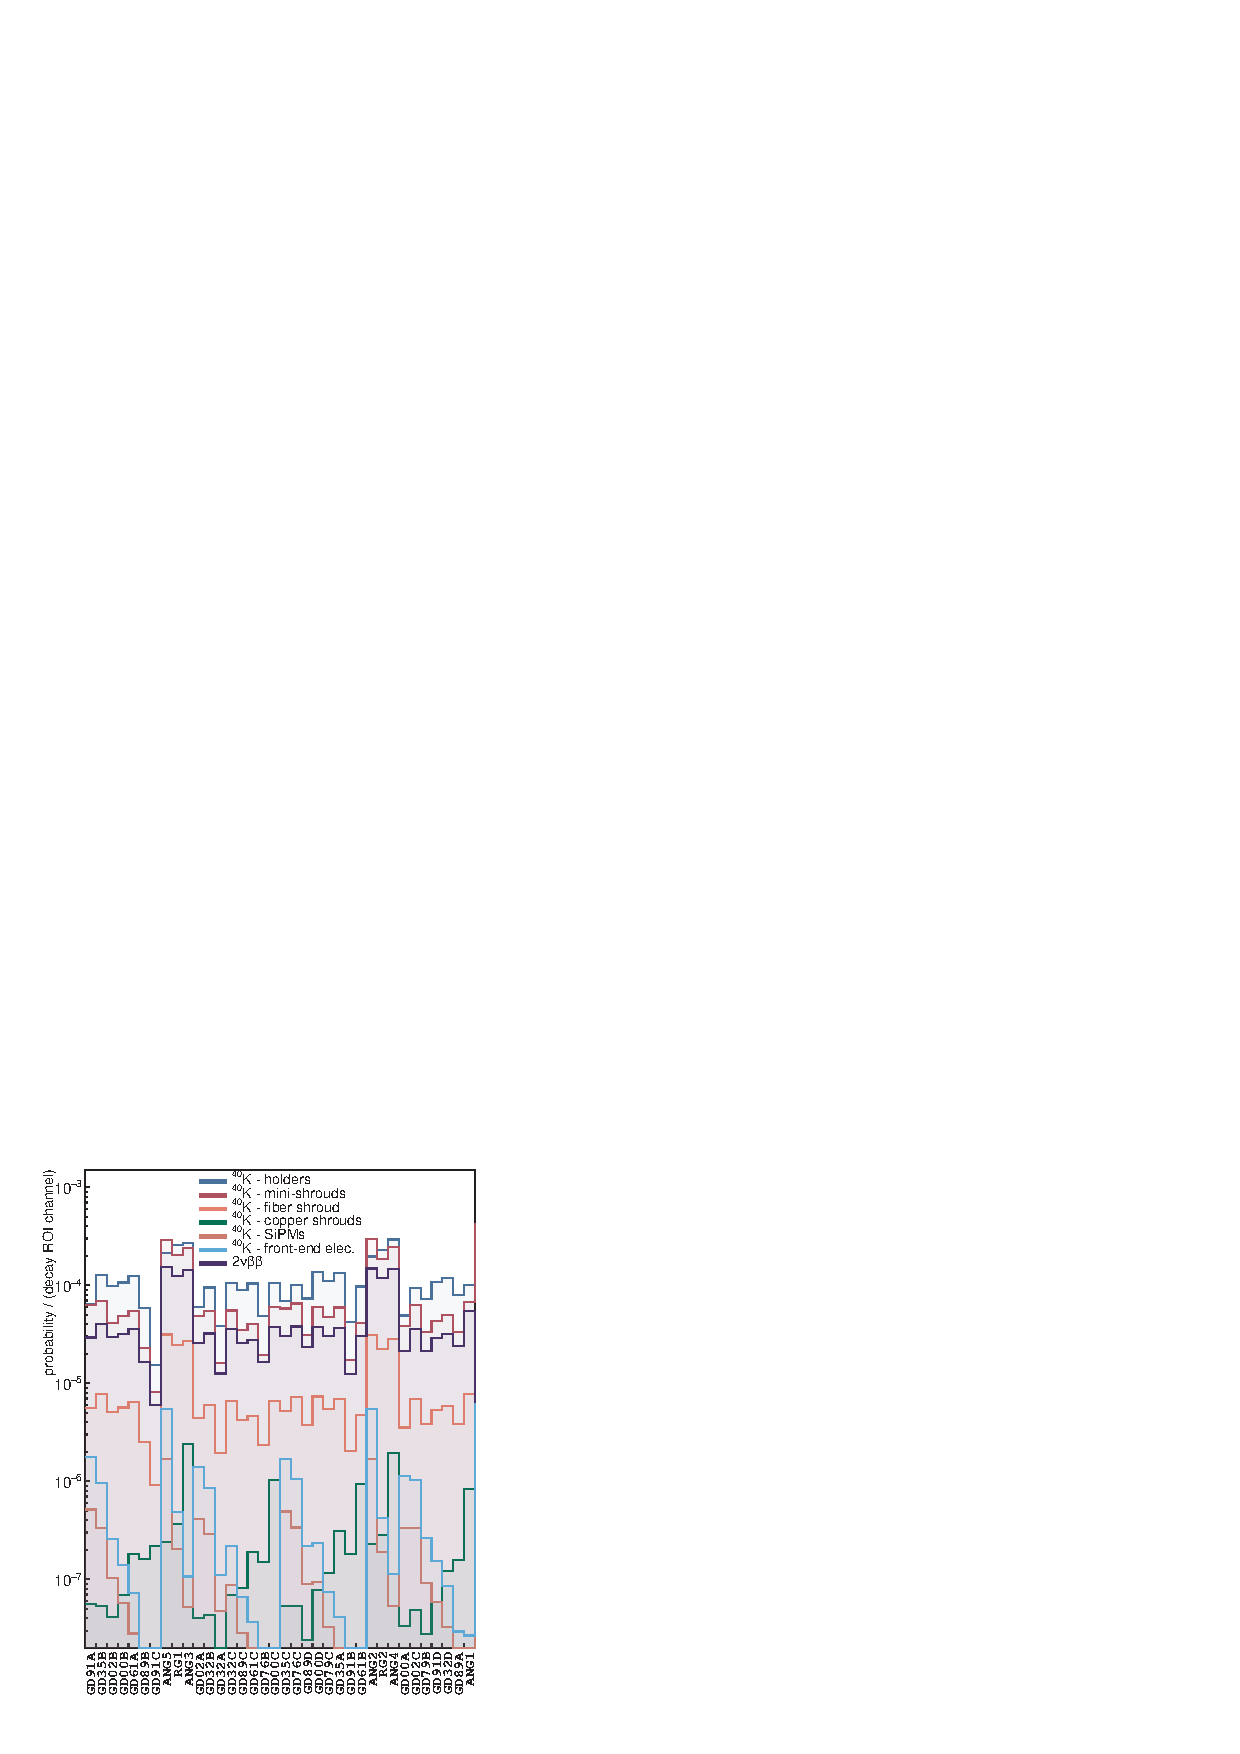
\includegraphics[width=0.48\textwidth]{plots/bkg/raw/ph2/pdfs/kmodel-pdfs-K40.pdf}}
  \hfill
  \subfloat[%
  \kvn\ located close to each single mini-shroud, \Mokvn\
  data set.\label{fig:bkg:raw:ph2:pdfs:kmodel:K40sep:M1}%
  ]{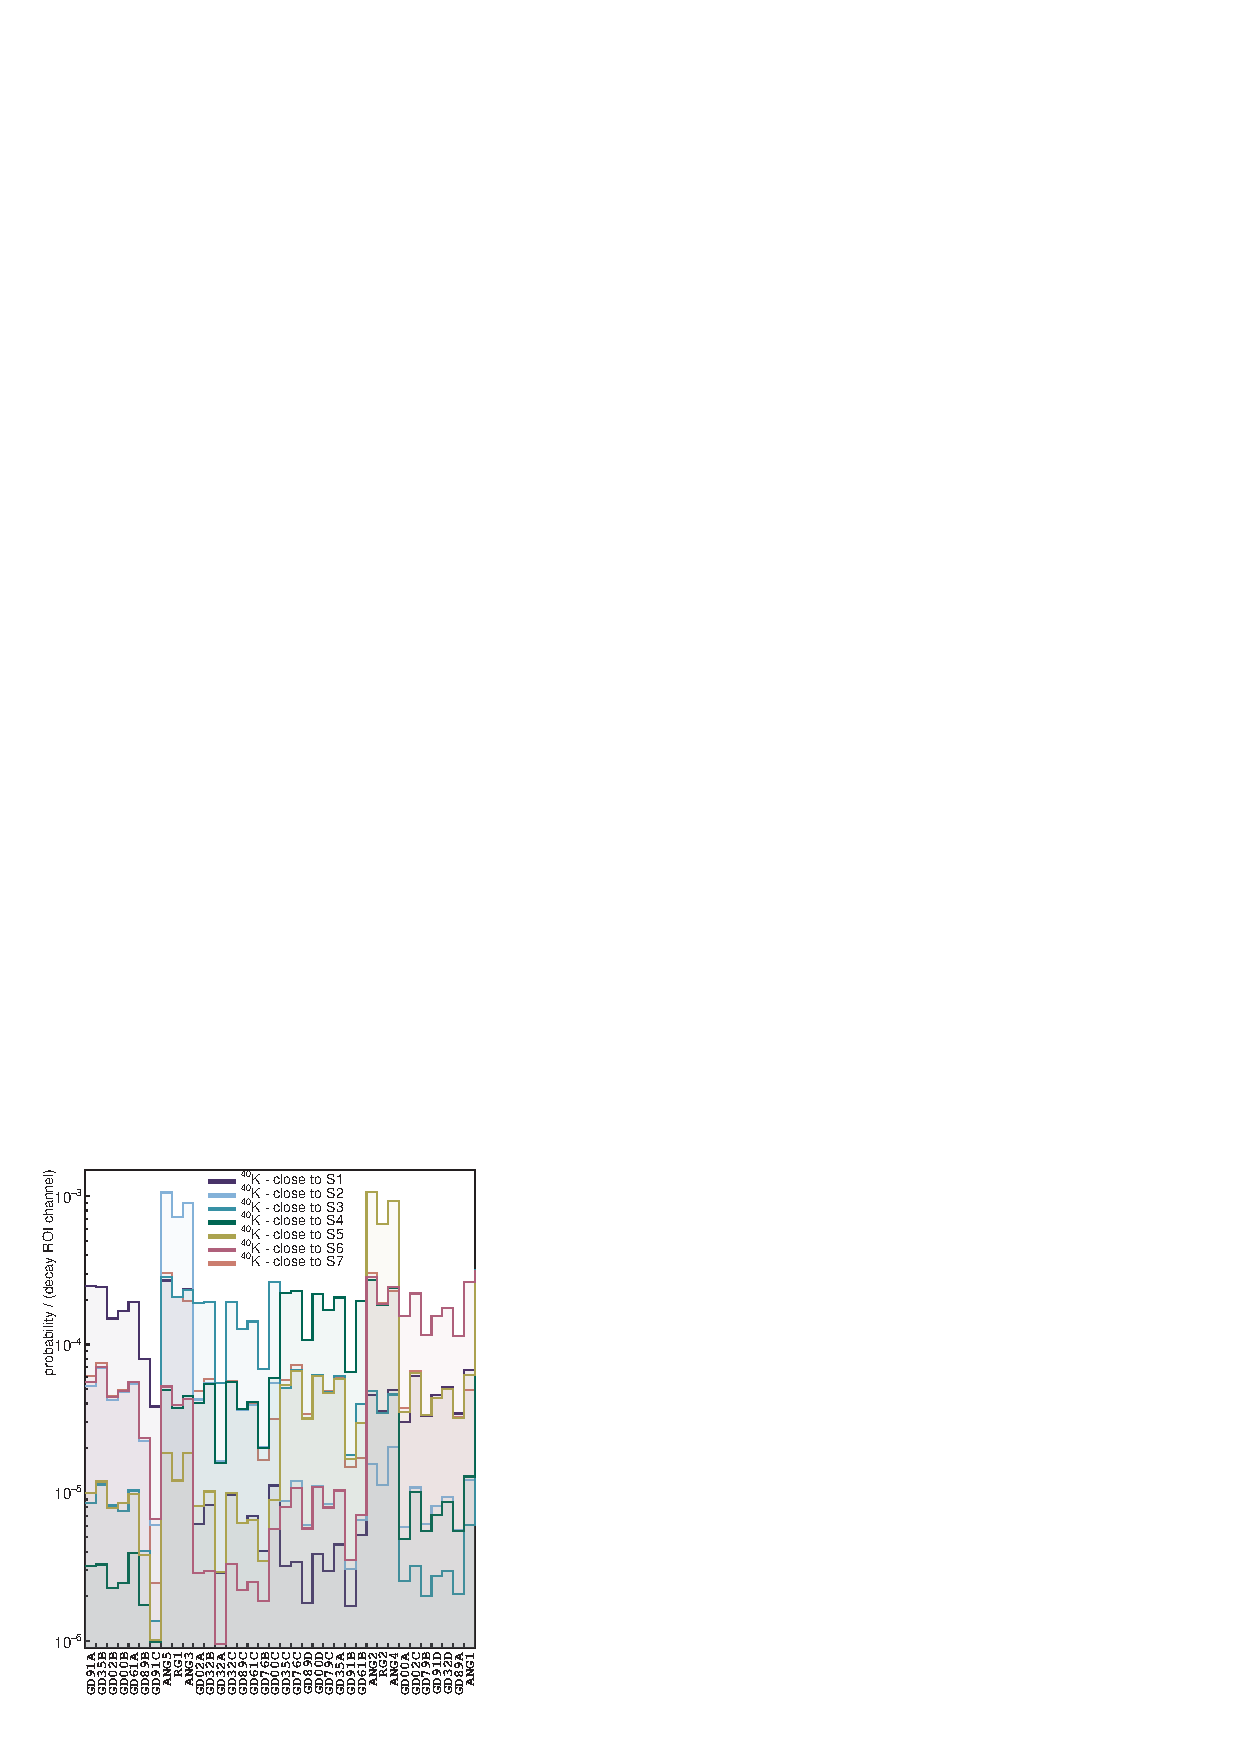
\includegraphics[width=0.48\textwidth]{plots/bkg/raw/ph2/pdfs/kmodel-pdfs-K40-sep.pdf}}

  \subfloat[%
  \kvn\ in different setup locations, \Mtkvn\
  data set.\label{fig:bkg:raw:ph2:pdfs:kmodel:K40:M2}%
  ]{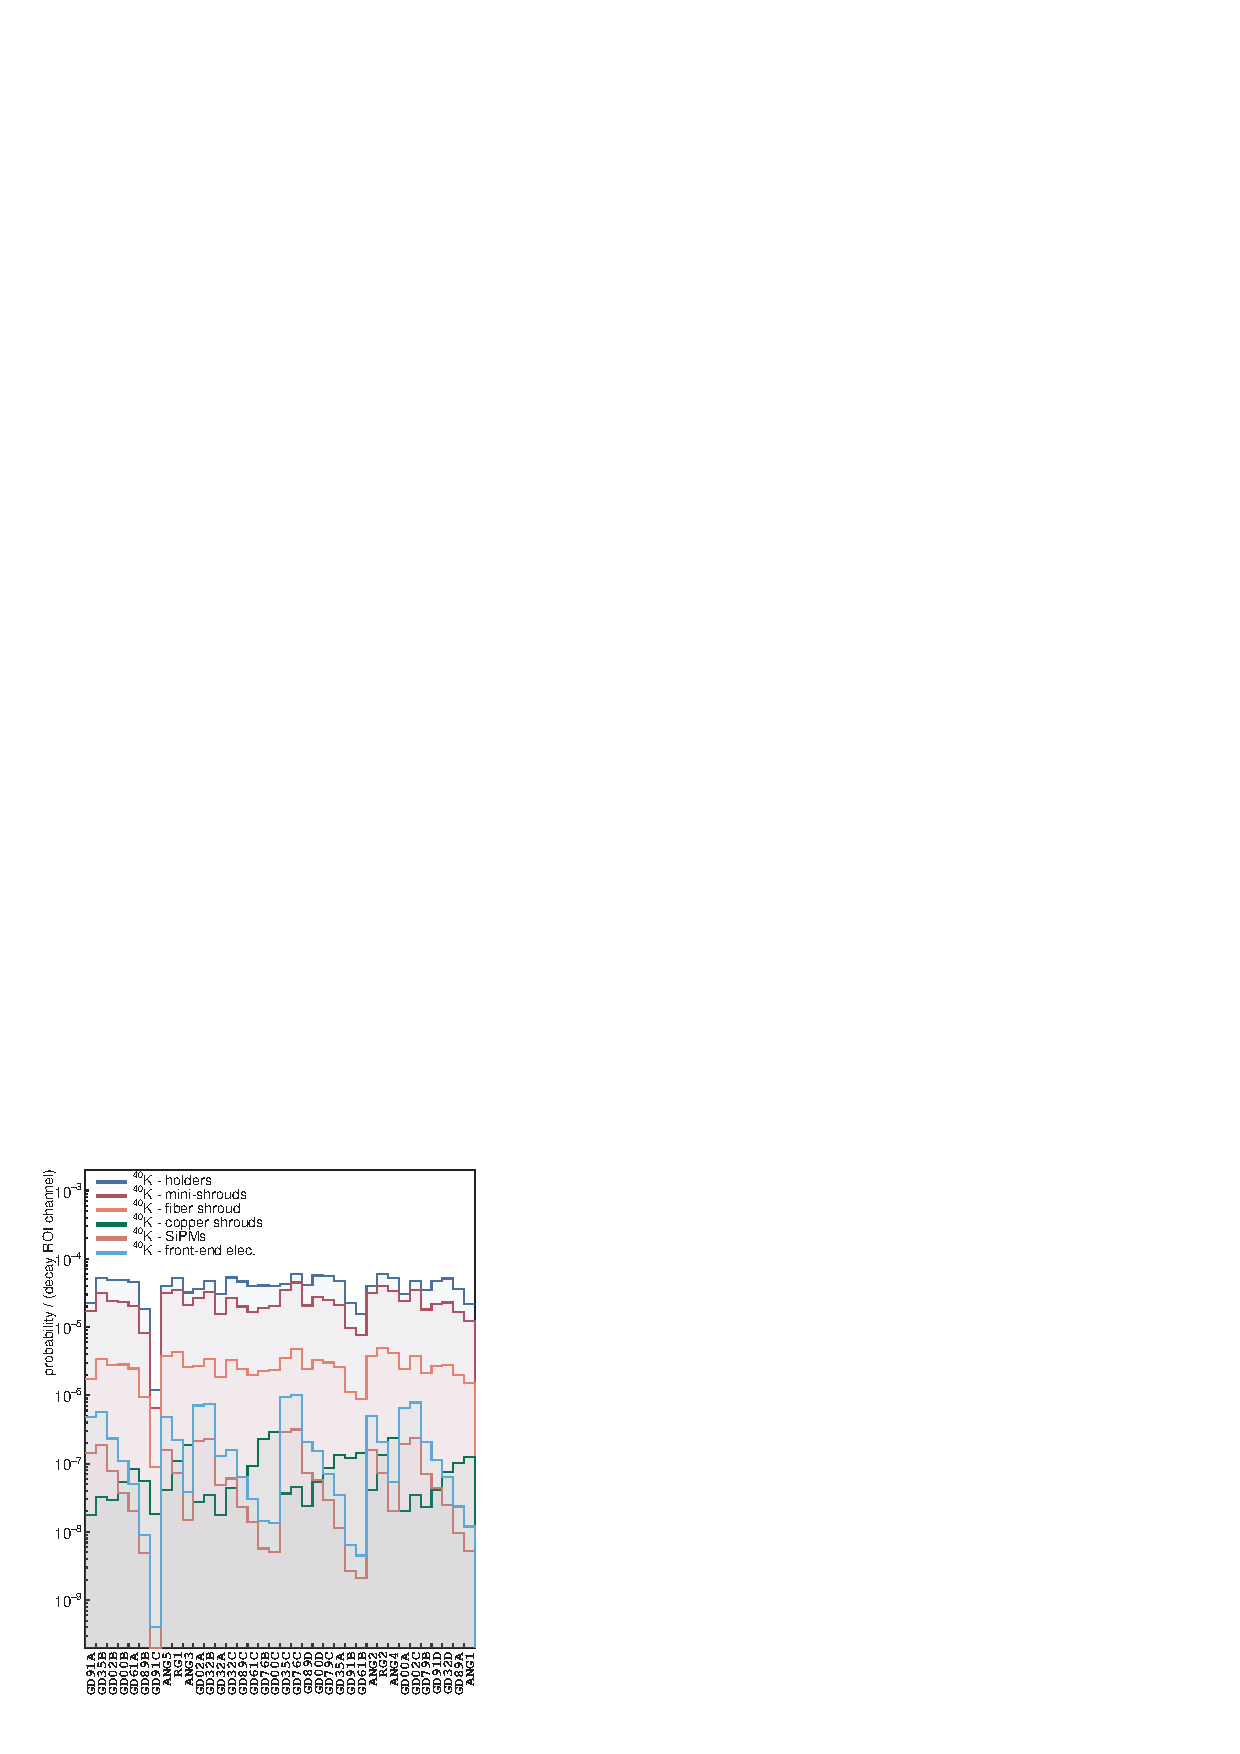
\includegraphics[width=0.48\textwidth]{plots/bkg/raw/ph2/pdfs/kmodel-pdfs-K40-M2.pdf}}
  \hfill
  \subfloat[%
  \kvn\ located close to each single mini-shroud, \Mtkvn\
  data set.\label{fig:bkg:raw:ph2:pdfs:kmodel:K40sep:M2}%
  ]{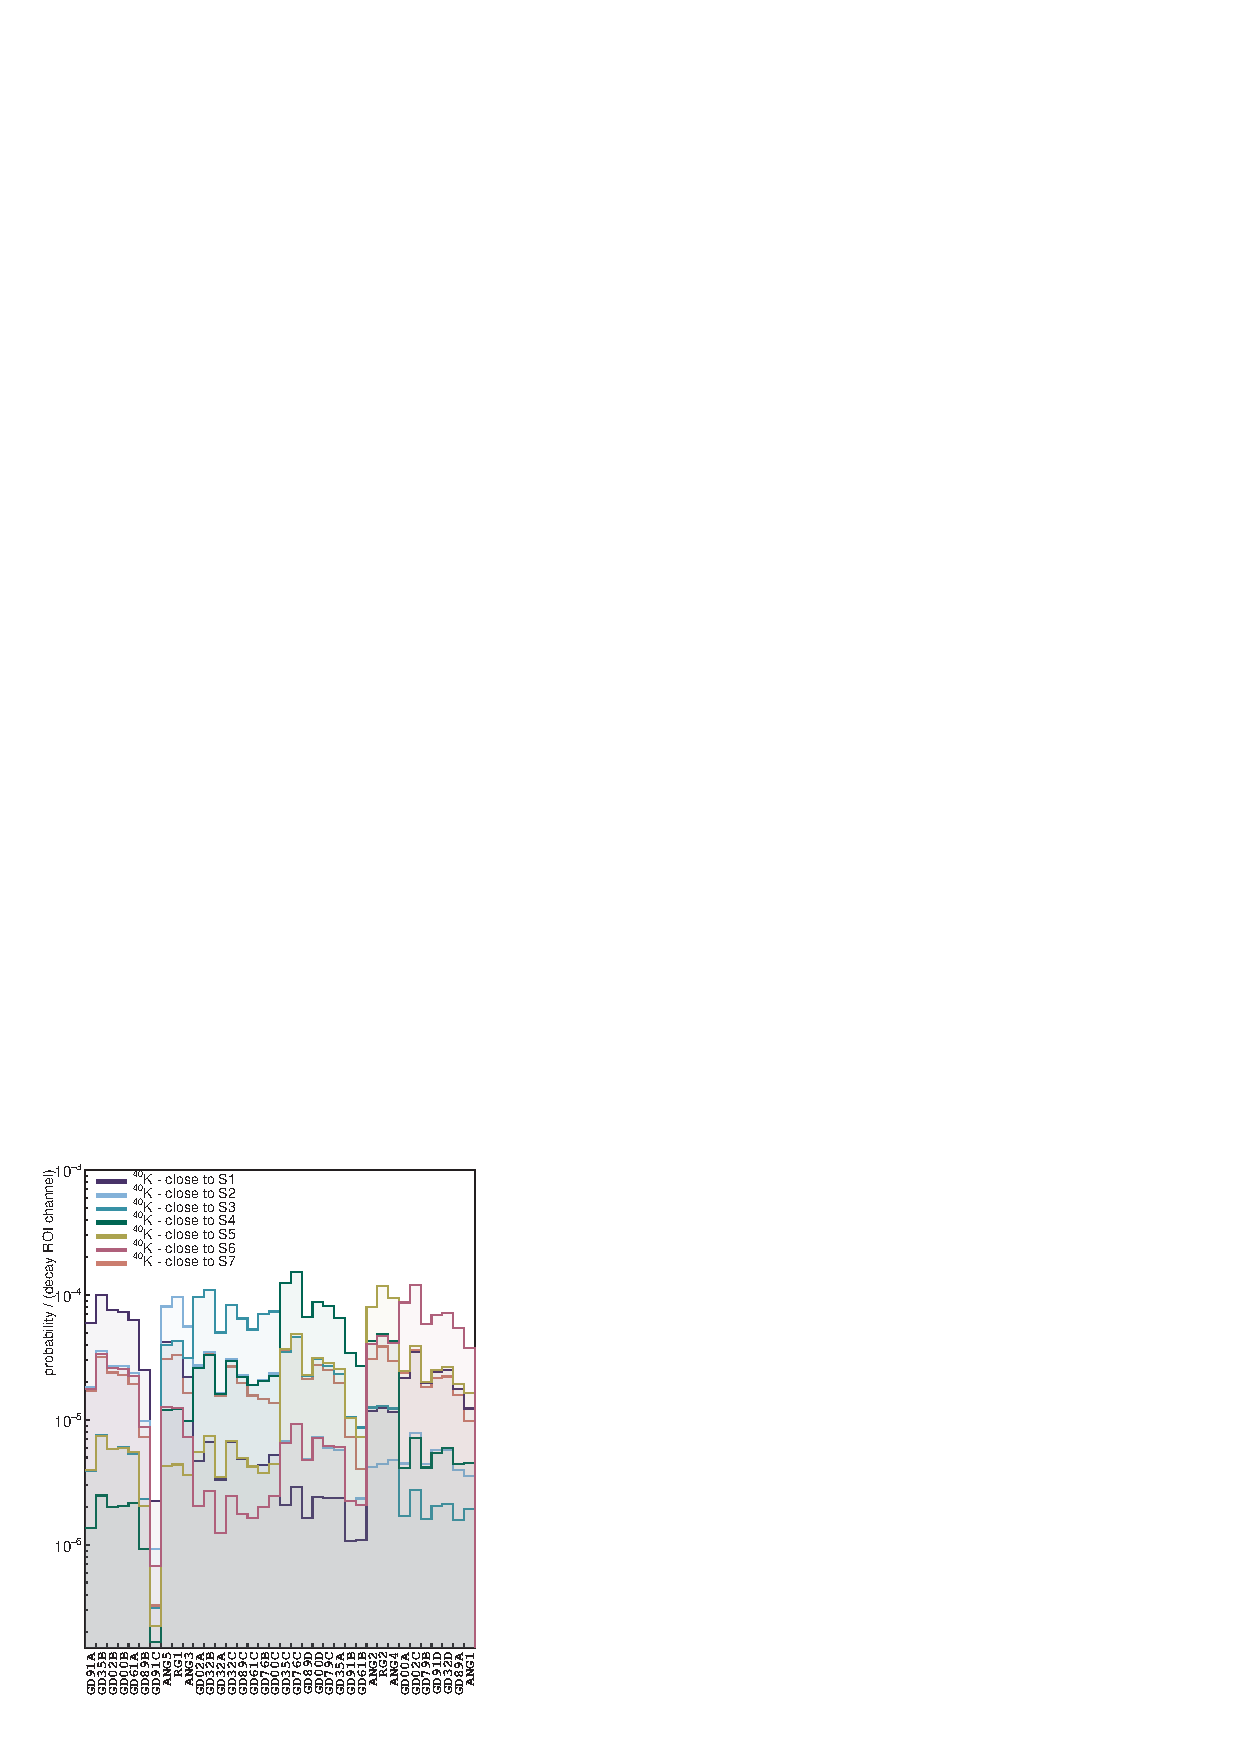
\includegraphics[width=0.48\textwidth]{plots/bkg/raw/ph2/pdfs/kmodel-pdfs-K40-sep-M2.pdf}}

  \caption{%
    \pdf{}s binned in detector space for the \kvn\ tracking analysis. 
    All \pdf{}s are normalized to the number of simulated primary decays.
  }\label{fig:bkg:raw:ph2:pdfs:kmodel:K40}
\end{figure}

\begin{figure}
  \subfloat[%
  \kvz\ in different setup locations and \nnbb\ in Ge,
  \Mokvz\ data set.\label{fig:bkg:raw:ph2:pdfs:kmodel:K42:M1}%
  ]{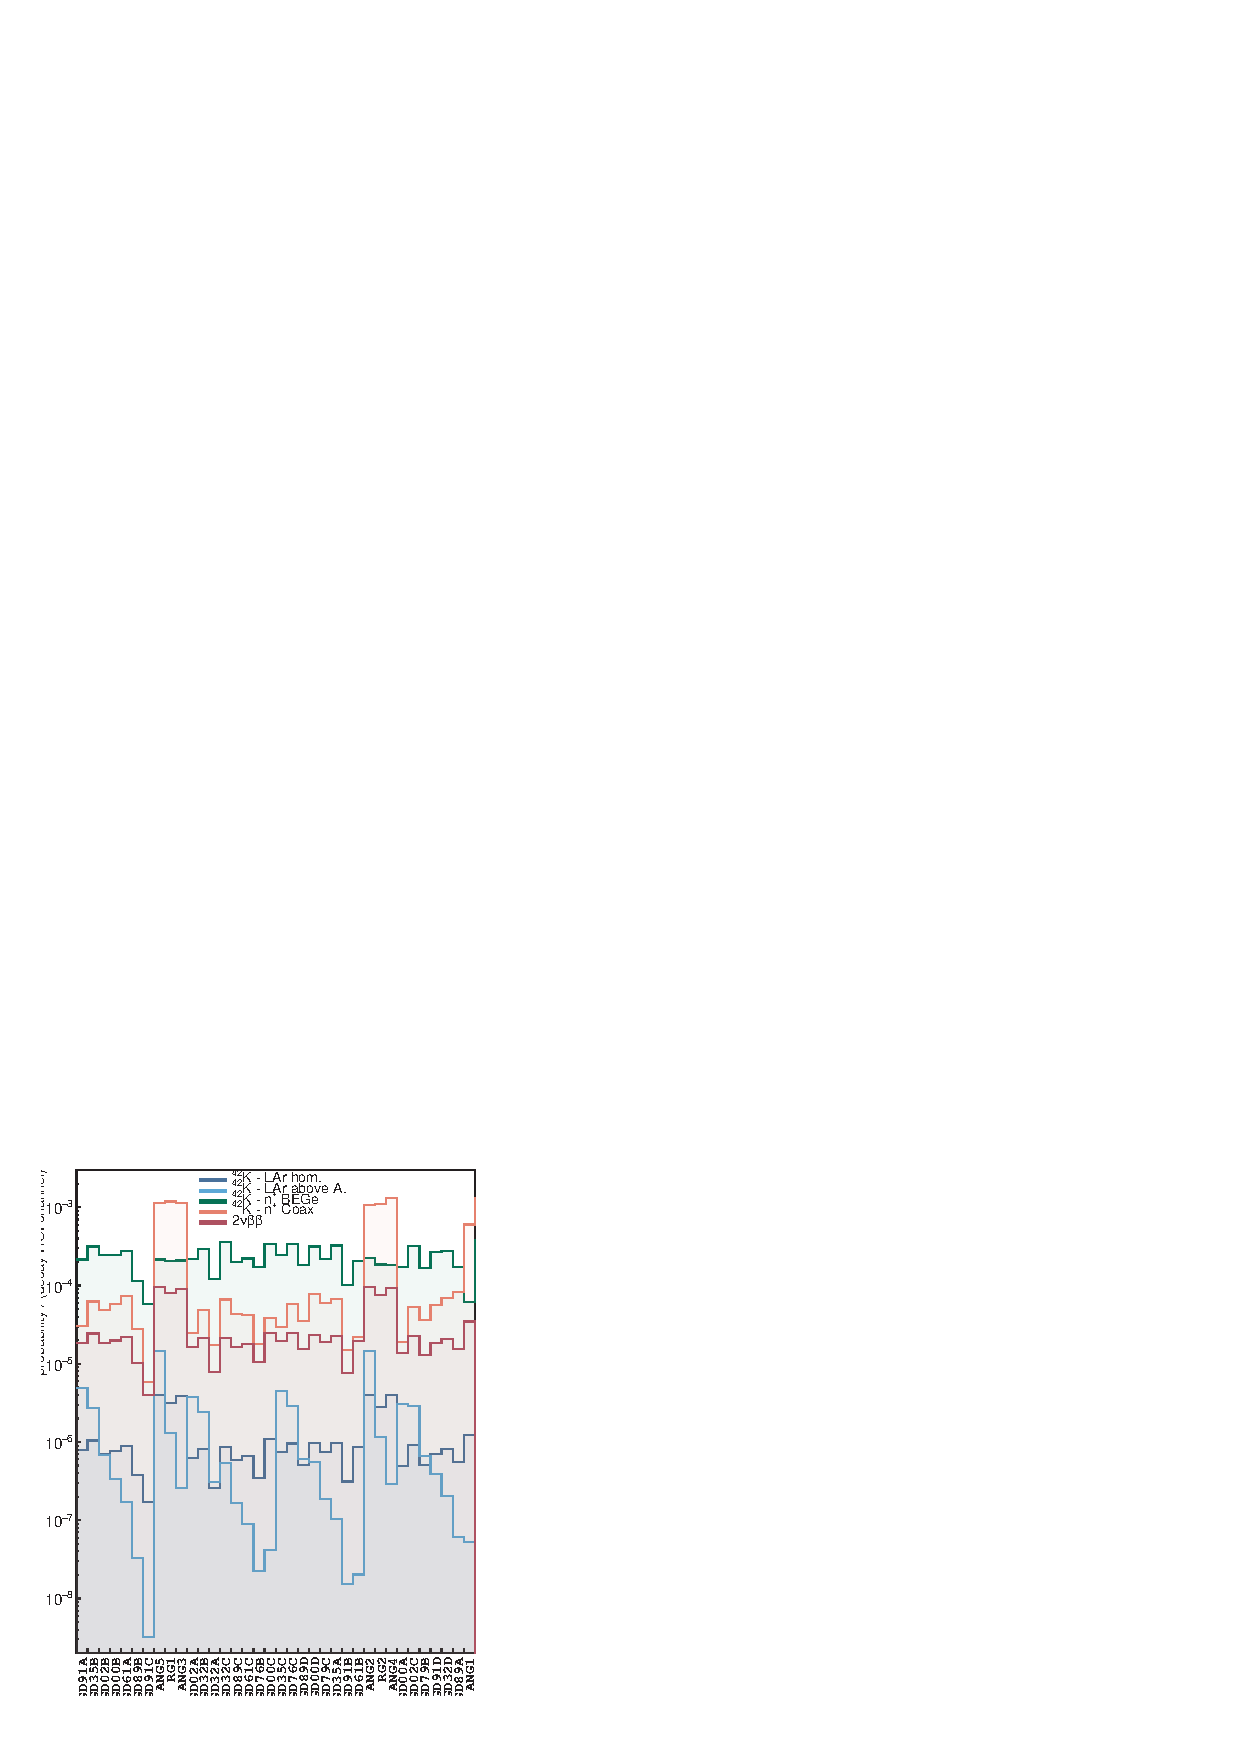
\includegraphics[width=0.48\textwidth]{plots/bkg/raw/ph2/pdfs/kmodel-pdfs-K42.pdf}}
  \hfill
  \subfloat[%
  \kvz\ in LAr above each single mini-shroud, \Mokvz\
  data set.\label{fig:bkg:raw:ph2:pdfs:kmodel:K42sep:M1}%
  ]{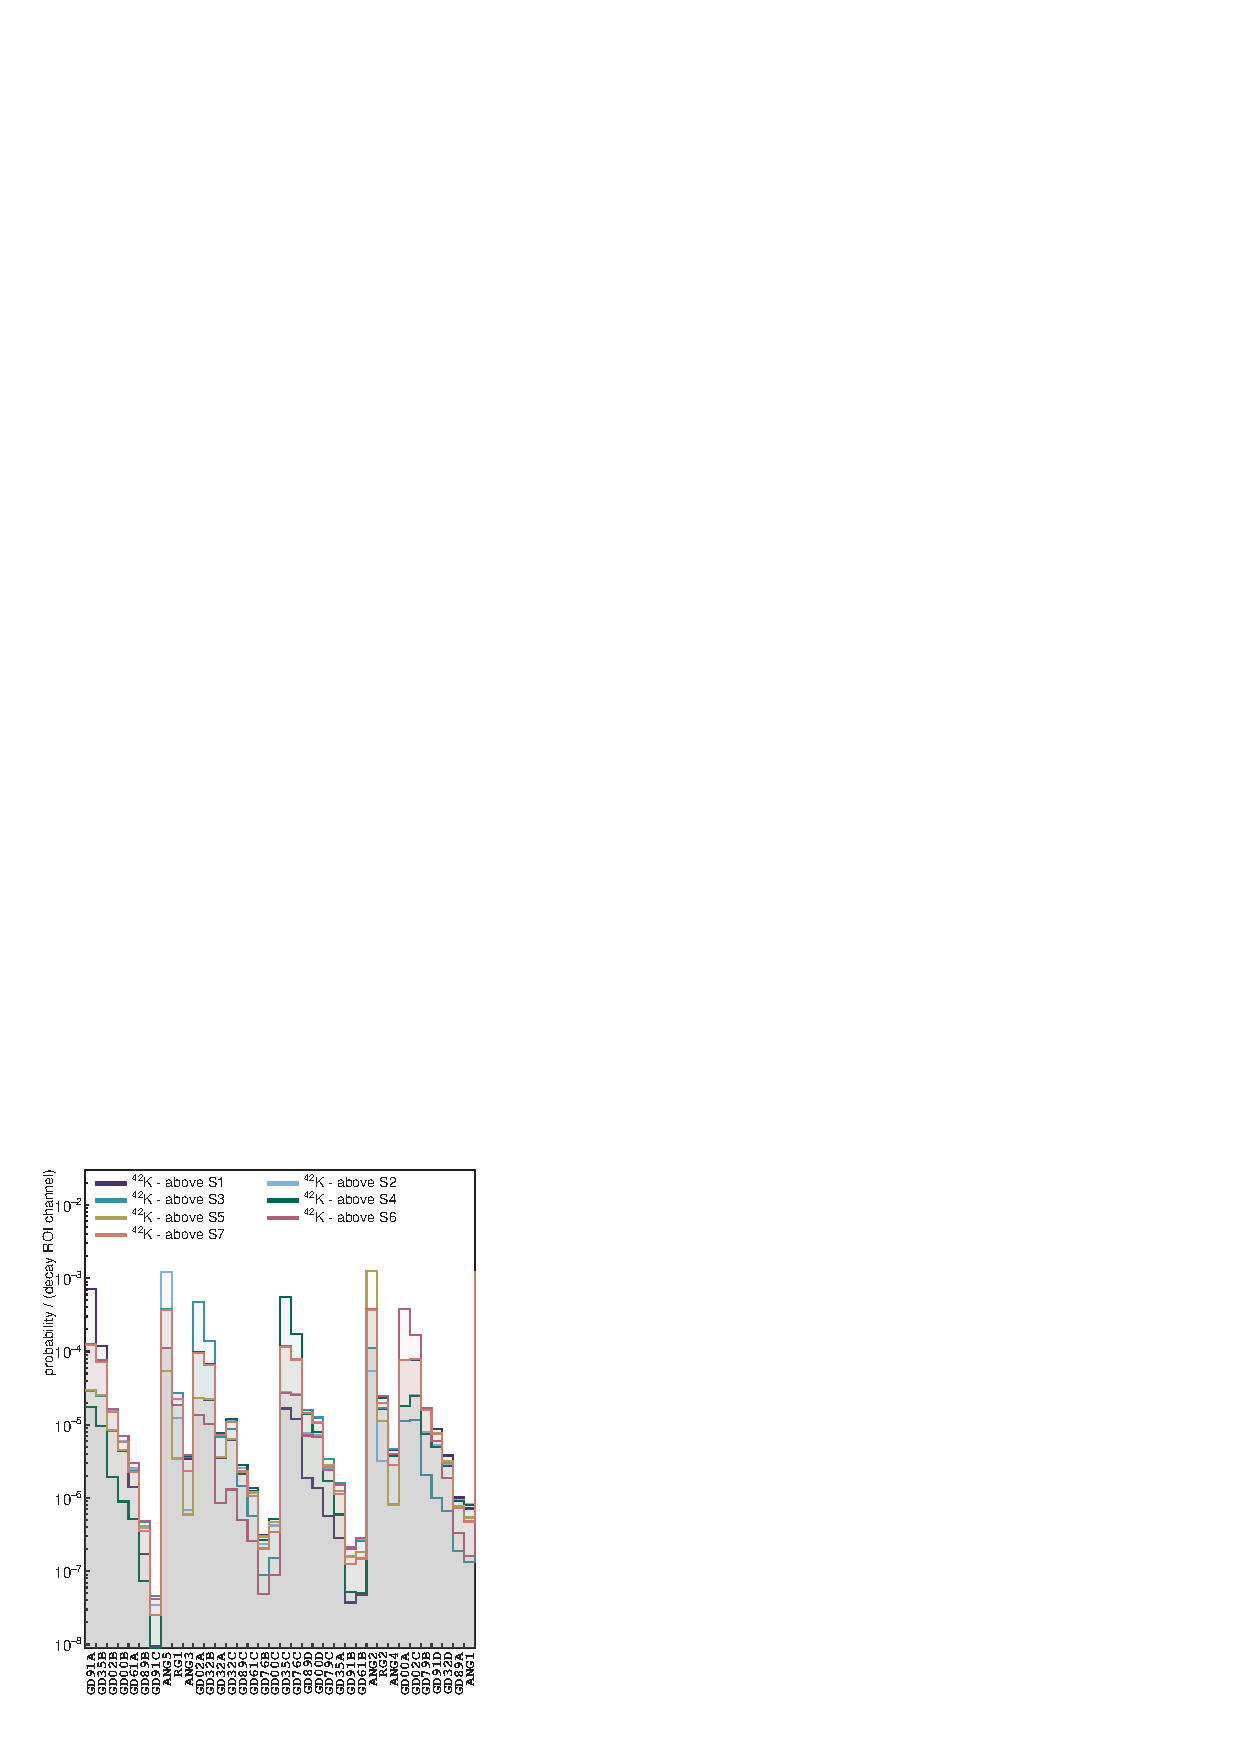
\includegraphics[width=0.48\textwidth]{plots/bkg/raw/ph2/pdfs/kmodel-pdfs-K42-sep.pdf}}

  \subfloat[%
  \kvz\ in different setup locations, \Mtkvz\
  data set.\label{fig:bkg:raw:ph2:pdfs:kmodel:K42:M2}%
  ]{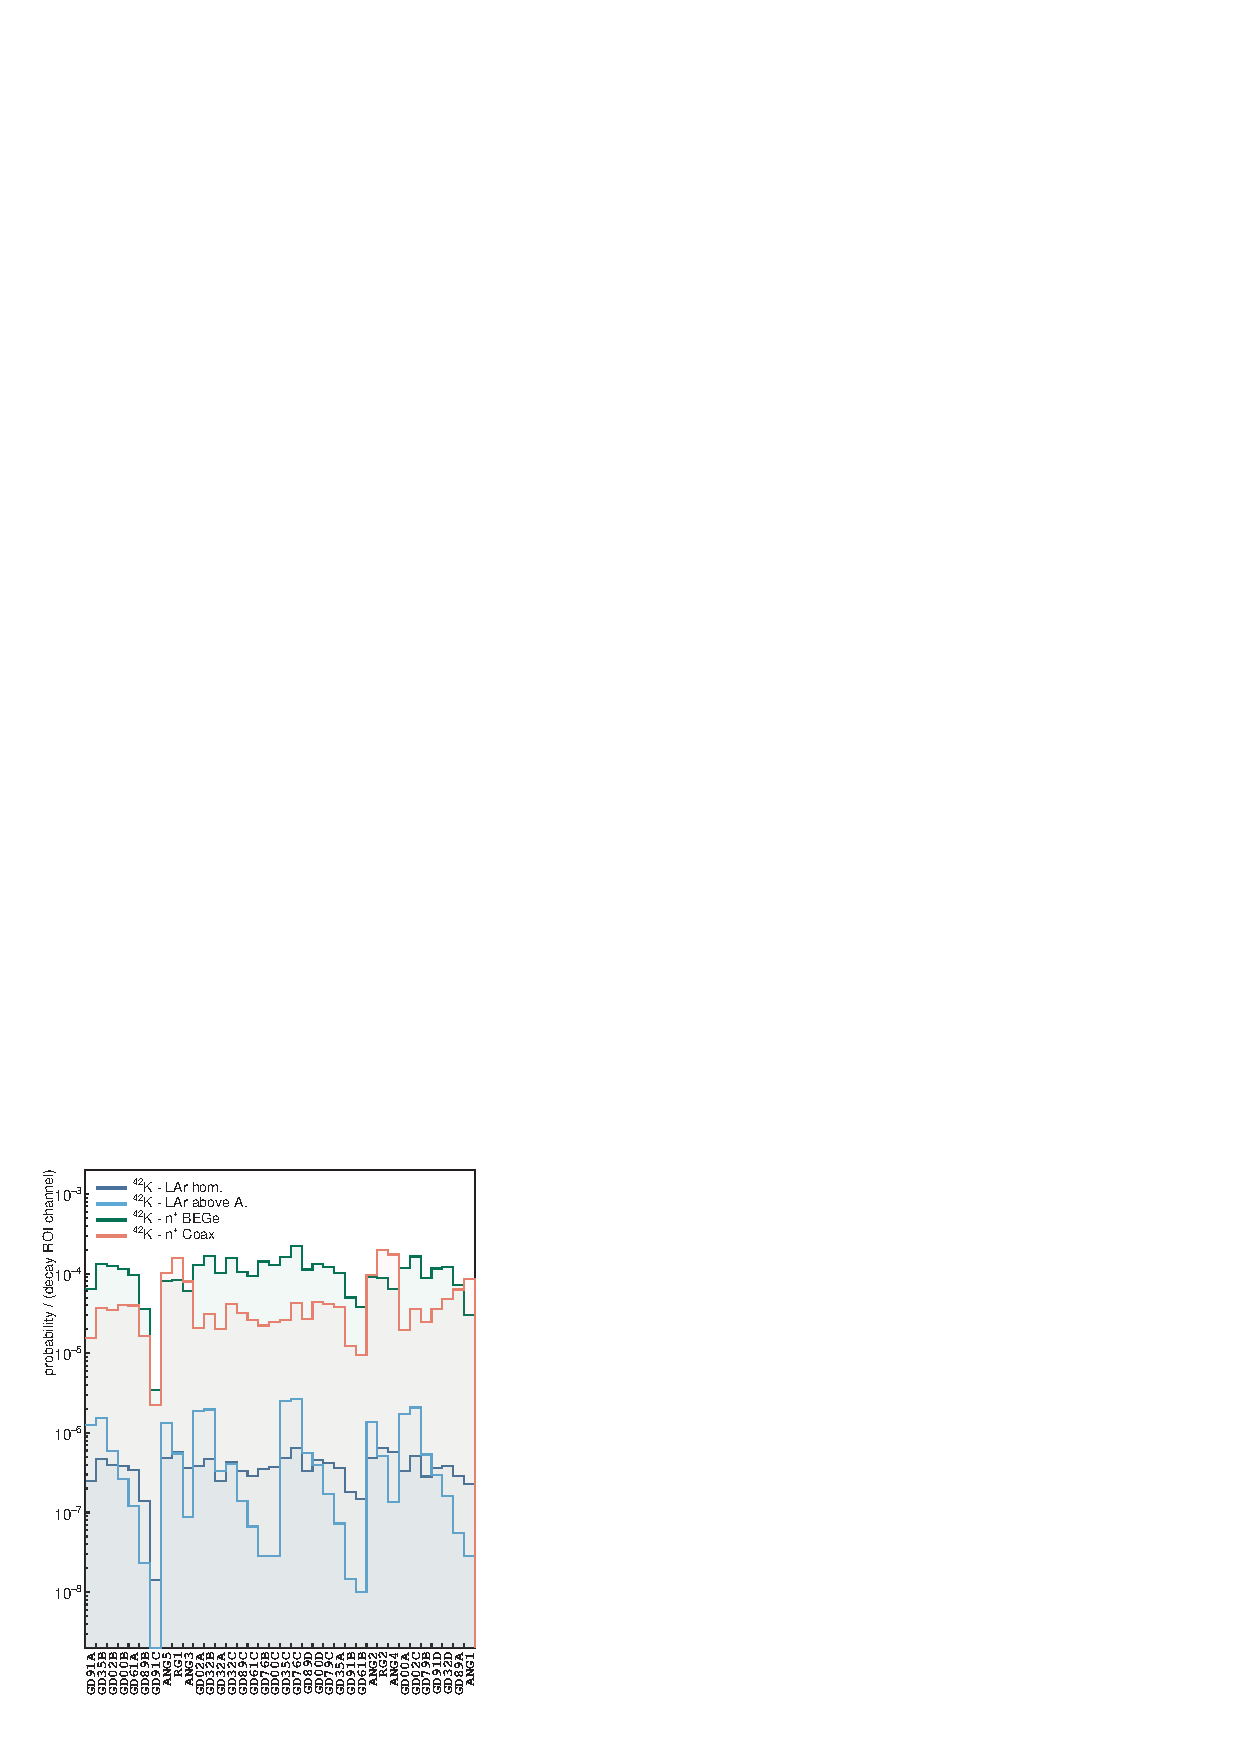
\includegraphics[width=0.48\textwidth]{plots/bkg/raw/ph2/pdfs/kmodel-pdfs-K42-M2.pdf}}
  \hfill
  \subfloat[%
  \kvz\ in different setup locations, \Mtkvz\
  data set.\label{fig:bkg:raw:ph2:pdfs:kmodel:K42sep:M2}%
  ]{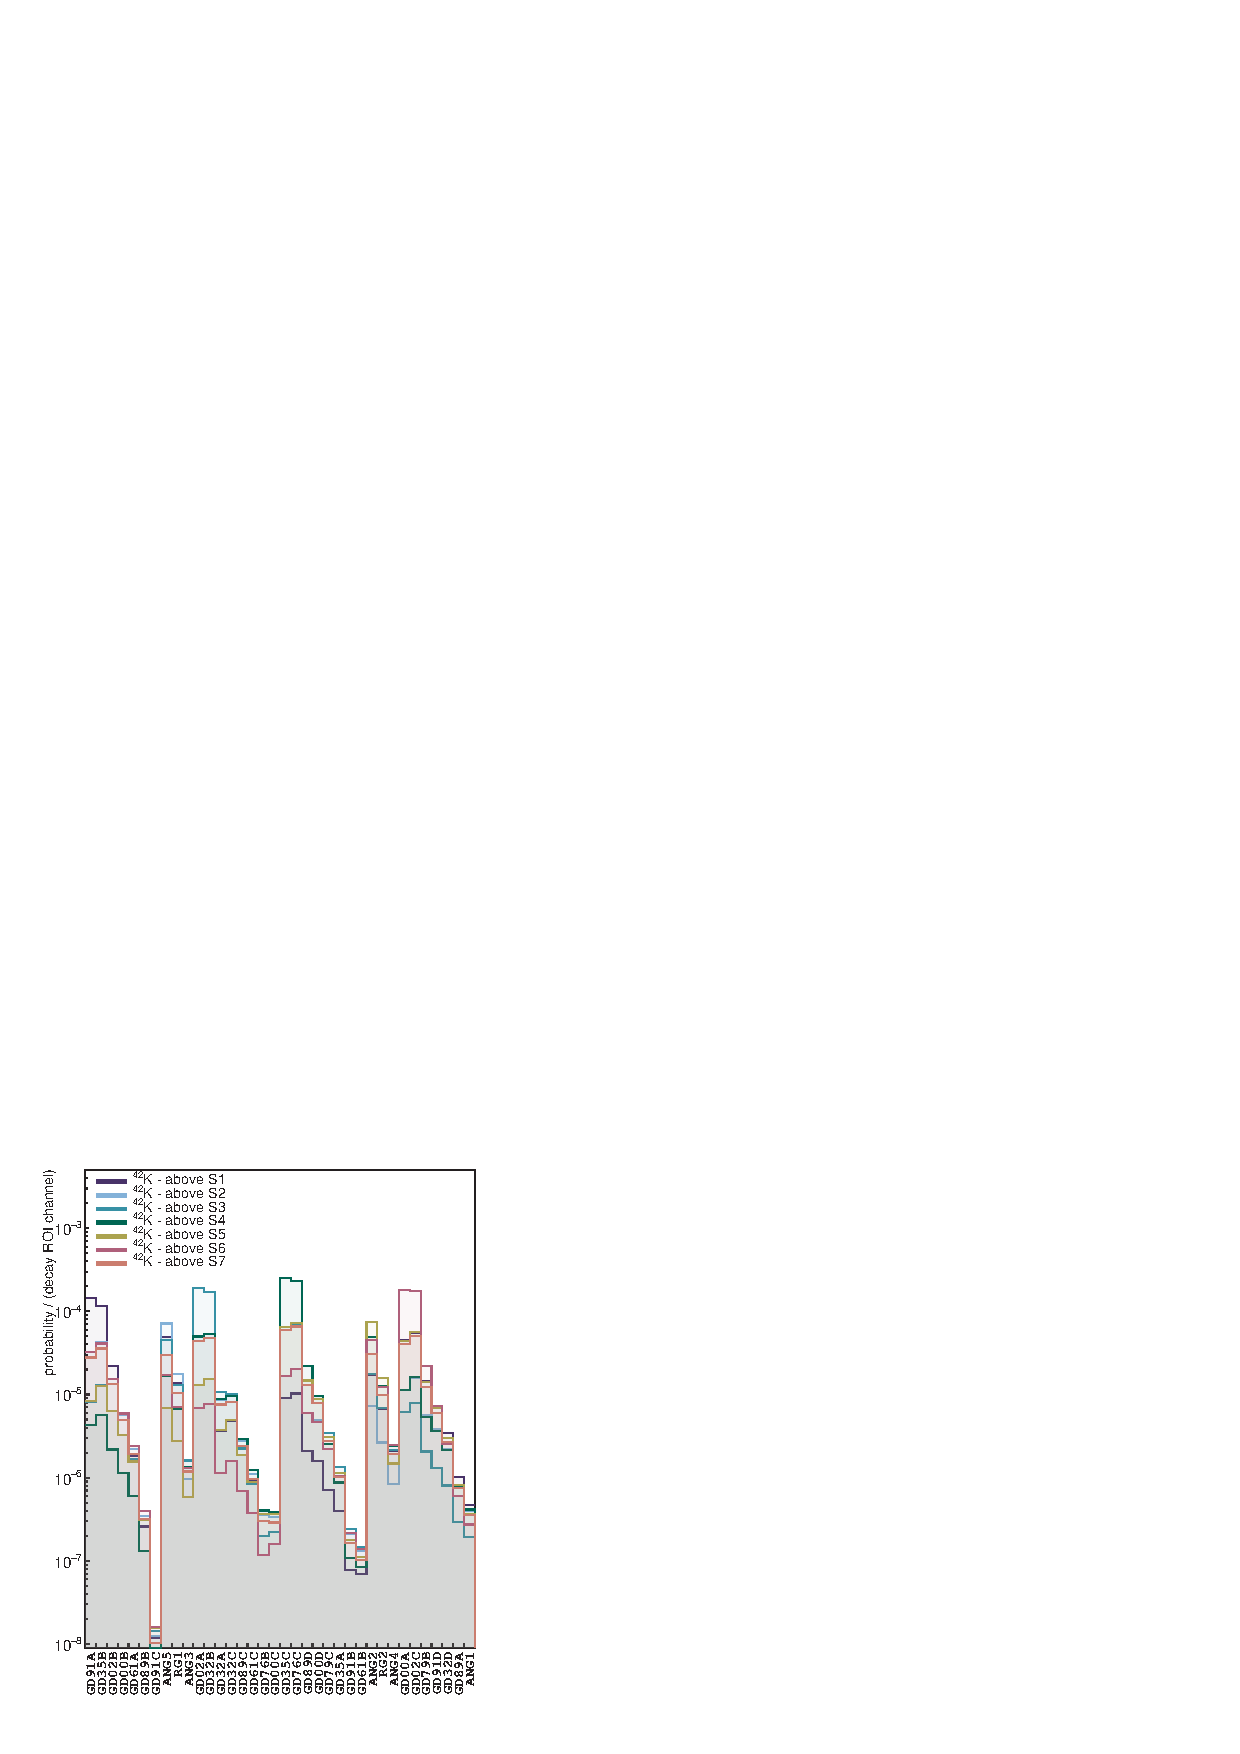
\includegraphics[width=0.48\textwidth]{plots/bkg/raw/ph2/pdfs/kmodel-pdfs-K42-sep-M2.pdf}}

  \caption{%
    \pdf{}s binned in detector space for the \kvz\ tracking analysis. 
    All \pdf{}s are normalized to the number of simulated primary decays.
  }\label{fig:bkg:raw:ph2:pdfs:kmodel:K42}
\end{figure}

\blocktitle{management \\ tools}
The \mage\ simulations are performed at the high-performance computing cluster of the Max
Planck Instutit f\"ur Kernphysik in Heidelberg (Germany), where access to a job queue (for
a maximum of 200 concurrent jobs per user) and several PB of disk space is granted.
Managing simulations and their post-processing queue is not a simple
task when scaling up significantly their number and size. As a reference, the \gerda\
simulation output saved on disk which is used to produce the background model \pdf{}s amounts
to about 30~TB of data. Moreover, simulations are split up in small chunks to allow for
parallelization of the workload and to not exceed the maximum run time per job allowed by
the job scheduler\footnote{%
  The Son of Grid Engine (\url{https://arc.liv.ac.uk/trac/SGE}), a community project to
  continue Sun's old grid engine previously used on the cluster, is used for allocating
  computing resources to users and running batch jobs.
}, resulting in about $\sim$$10^{5}$ files that need to be managed.
\newpar
The \mage\ simulations are stored in databases, which contain macro files (that configure
a simulation job and are directly fed into \mage), output files and log files organized
in a specific directory structure (i.e.~\m{group1/group2/isotope/subtype}). Multiple
separate databases can be managed at the same time (e.g.~to keep \phasetwo\ and
\phasetwop\ simulations separate). A library of code utilities\footnote{%
  The \m{GeMS.jl} (\gerda\ \mage\ Simulations) library is a
  Julia-based~\cite{Bezanson2017} toolkit with functions to analyze JSON simulation
  databases, populate them with \mage\ macros and interact with a SGE job scheduler.
  Management of large databases is efficiently automated, providing a simple user
  interface to check whether macros should be written or updated or outdated simulations
  should be re-run. Support for parallel processing is available. \m{GeMS.jl} is part of
  the \m{gerda-gems-sw} software stack available on GitHub at
  \url{https://github.com/mppmu/gerda-gems-sw}.
} has been developed to automate the interaction with the job scheduler and populate the
database with simulation output. The database is built through a JSON-based metadata
interface. The user is required to specify the simulation parameters (including the \mage\
volume in which the primaries should be confined, the number of simulated events, the
number of parallel jobs, the commands required to define the physics of the simulation,
the software version, etc.) by filling \m{metadata.json} files, which are subsequently
parsed by the \m{GeMS.jl} software when populating the database with macro configuration
files. The following part of metadata file, for example, defines the volume used to
simulate radioactive contaminations in the cabling (\m{cables/cables\_all}):
\begin{lstlisting}[language=json, style=jsonstyle]
{
    "cables": {
        "template": "gerda-ph2",
        "cables_all": {
            "description": "All the cables parts together, HV, signal and the cable patches",
            "simulated-properties": {
                "mass-g": 31.01,
                "volume-cm3": 20.26,
                "density-gcm3": 1.53
            },
            "mage-volumes": [
                "HVCableAtHolder_Phase2_[0-39]",
                "SignalCableAtHolder_Phase2_[0-39]",
                "HVCableFromHolderToElectronicsPlate_Phase2_[0-39]",
                "SignalCableFromHolderToElectronicsPlate_Phase2_[0-39]"
            ]
        },
        // ...
    }
}
\end{lstlisting}
The following excerpt configures a \kvn\ simulation in the cables.
\begin{lstlisting}[language=json, style=jsonstyle]
{
    "cables": {
        "cables_all": {
            "K40": {
                "additional-commands": {
                    "generator": [
                        "/MG/generator/select G4gun",
                        "/MG/generator/g4gun/cone_on true",
                        "/gun/particle ion",
                        "/gun/ion 19 40",
                        "/gun/energy 0 eV"
                    ]
                },
                "edep": {
                    "mage-version": {
                        "revision": "gerda-v2.0.0-rc3",
                        "gerda-sw-all": "gerda-sw-all_v6.1.1-mage@gerda-v2.0.0-rc3"
                    },
                    "total-events": 1.0e9,
                    "number-of-files": 100,
                    "contact": "L.Pertoldi"
                }
            },
            // other isotope...
        }
    }
}
\end{lstlisting}
In this way, the user is absolved from having to deal with thousands of files and
the database can be versioned with Git\footnote{\url{https://git-scm.com}}. Databases for
background model simulations are uploaded to
GitHub\footnote{\url{https://github.com/mppmu/gerda-gems-db}}.
\newpar
The simulation post-processing to obtain the background \pdf{}s is also managed with the
cluster job scheduler and dedicated automation software tools\footnote{%
  Available on GitHub at \url{https://github.com/mppmu/gerda-pdfs}.
}. Each single simulation has to undergo a process pipeline to fold detector parameters
and run-dependent information into the raw \mage\ output, before being parsed by histogram
generation routines that write the \pdf{}s to disk. The software utilities interact with the
job scheduler and add the requested or outdated jobs to the queue, based on the set of
simulations selected by the user. The letter is required to provide a list of simulations
as input; the software then builds a local replica of the database with symbolic links to
the corresponding directories in the simulation database and inspects it. The \pdf\
production is also configured with JSON files; the detector active volume parameters, the
energy calibration and all other settings can then be modified by the user without any
need to recompile the software. The ROOT files with the output \pdf{}s are then distributed
to the collaboration.
\newpar
The reproducibility of the results is guaranteed in various ways. First, the simulation
databases and the software are versioned with Git. Once a new \pdf\ release is ready, it is
distributed with a progressive version number, and the software revision is tagged. The
\pdf\ production configuration files are shipped as part of the \pdf\ release. Lastly, all the
simulation and \pdf\ production pipeline is run within Singularity~\cite{Kurtzer2017,
Singularity2020} containers.

\section{Optical physics in \mage}%
\label{sec:apdx:mage-optics}

The computation of the LAr veto flag for Monte Carlo events is described
in~\cref{sec:bkg:lar:ph2:heatmap}. Here, a reference list of the optical properties
implemented in \mage\ that regulate the propagation of light in the \gerda\ cryostat is
given.
\newpar
Optical materials and surfaces are implemented in \mage\ through the relevant \geant\
libraries. Once properties like reflectivity, wavelength-shifting capabilities,
attenuation lengths, scintillation yields etc.~are defined, the \geant\ core routines take
care of simulating light propagation accordingly. When defining optical parameters in the
Monte Carlo, one must keep in mind what are the typical photon wavelengths that come to
play in the \gerda\ setup. The most important wavelength is 128~nm, in the so-called
vacuum-ultra-violet (VUV) regime, which defines the energy of the photon emitted by the
LAr scintillation process. The second interesting regime is in the 400--600~nm range,
typical of photons which are wavelength-shifted (WLS) in the fiber curtain or by
Tetraphenil-Butadiene (TPB) coatings to match the absorption range of the light detectors
(PMTs, SiPMs). As it will be clear in the next sections, many optical parameters are
poorly known in the VUV regime or depend on the details of the experimental setup (LAr
purity, WLS coating thickness etc.), and a dedicated measurement should be therefore
performed. In the following a reference list of the optical properties implemented in
\mage\ is provided, with references to the literature.

\blocktitle{liquid \\ argon}
Key properties of the liquid argon from the point of view of the vetoing performance in
\gerda\ are the scintillation mechanism, the refractive index and the attenuation length.
The first two are relatively well known, while the latter strongly depends on the LAr
purity, which has not been measured for \gerda. We recall here that the deployed LAr has
not been subject to any purification process, and is therefore expected to meet the purity
specifications of natural argon.

\begin{description}

  \item[Refractive index] Its implementation depends on the photon energy (shown in
    \cref{fig:bkg:lar:ph2:mage:lar-props}). Formulas are taken from~\cite{Bideau-Mehu1981}
    and give about 1.41 at 128~nm. A more recent measurement, similarly based on an
    extrapolation of measured data to lower wavelengths, suggests a lower value of about
    1.37~\cite{Babicz2018}.

  \item[Rayleigh scattering length] Depends on the refractive index and therefore the
    photon energy (shown in \cref{fig:bkg:lar:ph2:mage:lar-props}). Formulas are taken
    from~\cite{Seidel2002}. The already implemented refractive index values are used. The
    obtained scattering length value at 128~nm is about 60~cm. The value suggested
    in~\cite{Babicz2018} is 91~cm, 50\% higher.

  \item[Scintillation spectrum] Taken from~\cite{Heindl2010}, which reports an
    experimental measurement (figs.~1 and 2). Only the (gaussian) peak is implemented in
    \mage, as the non-gaussian contributions are of several orders of magnitude lower and
    are therefore negligible. A normal distribution $(\mu=128\;\text{nm},
    \sigma=2.929\;\text{nm})$ is implemented (\cref{fig:bkg:lar:ph2:mage:lar-props}).

  \item[Scintillation yield] Different scintillation processes are defined in the \mage\
    physics list for different ionizing particles, that in general have different
    scintillation yields in LAr. A nominal value of $51\;\upgamma/\text{keV}$ is
    recommended in~\cite{Doke2002, Doke1988} for flat-top particles, which reduces to
    $40\;\upgamma/\text{keV}$ for \b\ and \g\ particles. This value does certainly not
    represent the reality of \gerda, as the yield strongly depends on the electric field
    configuration and the quencher impurity level. Unfortunately a reliable direct measure
    of the scintillation yield of the \gerda\ LAr is not available. Indirect measurements
    were performed within the \LArGe\ setup~\cite{Lehnert2016} and with a dedicated setup
    deployed inside the \gerda\ cryostat~\cite{Barros2020}, but they both yield
    incompatible results. A tentative, default value of 28~$\upgamma/\text{keV}$ for \b\
    and \g\ particles is implemented in \mage, which is the maximum achievable
    scintillation yield corresponding to 1~\mus\ triplet lifetime\footnote{%
      in first order, only the long-lived triplet state is affected by contaminant-induced
      non-radiative de-excitation. Electromagnetic interactions have a singlet-to-triplet
      ratio of 0.3~\cite{Doke2002}. The integral over the triplet decay for nominal
      1.6~\mus~\cite{Doke2002}, compared to the 1~\mus\ measured in \gerda\ (see
      \cref{fig:lar:triplet-lifetime}), gives a reduction of the light yield of $(0.3 +
      1/1.6)/1.3 = 71\%$. This estimate neglects impurities that affect the primary
      excimer production.
    }.
    As shown in~\cite{Doke2002}, some particles (in particular \a\ particles and nuclei)
    can be characterized by lower yields. Therefore, the photon yield is reduced for \a\
    particles and nuclei by a factor of 0.875 and 0.375 respectively in the physics list.
    These numbers are extracted from~\cite{Doke2002}. In this way \b\ and \g\ particles
    will be affected by the nominal (maximum) photon yield, while \a\ particles and nuclei
    will produce less light by a factor 0.875 and 0.375 (0.7/0.8 and 0.3/0.8 according
    to~\cite{Doke2002}), respectively.

  \item[Singlet and triplet lifetime] \sloppy The implemented triplet lifetime is the one
    measured during \gerdatwo, before the \phasetwop\ upgrade
    (\cref{fig:lar:triplet-lifetime}), the singlet lifetime is about 6~ns. The relative
    occurrence of the two de-excitation processes is also specified in terms of
    scintillation yield. The \geant\ \m{YIELDRATIO} property, which is defined as the
    relative strength of the fast component as a fraction of total scintillation yield, is
    set to 0.23 for all particles (\b\ and \g\ particles), 0.75 for nuclei and 1.0 for \a\
    particles (the latter is a rough guess).

  \item[Attenuation length] As the absorption length is strongly dependent on the LAr
    purity, no literature values can be used. It is known to depend on the wavelength of
    the photon in general, but this dependence is poorly known in the VUV regime. What is
    most important in \mage\ is its value at 128~nm, i.e.~the wavelength of the LAr
    scintillation light. The following, heuristic implementation is adopted: an
    exponential function is used to make sure that the LAr is opaque to VUV photons
    ($\lambda \leq 128$~nm) but transparent to wavelength-shifted photons ($\lambda
    \gtrsim 400$~nm), see fig.~\ref{fig:bkg:lar:ph2:mage:lar-props}. A measurement of the
    attenuation length in the \gerda\ LAr was performed~\cite{Barros2020}, yielding
    $\sim15$~cm as a result, but the performance of the LAr veto as well as recent
    measurements point towards larger absorption length. A default, reasonable value of
    55~cm is thus implemented in \mage\ and used in the LAr veto system simulation as
    `best guess'.

  \item[Fano factor] A Fano factor of 0.11 is set, taken from~\cite{Doke1976}.

\end{description}

\begin{figure}
  \centering
  \includegraphics{plots/mage/lar-props.pdf}
  \caption{%
    LAr optical properties as implemented in \mage. Top left: the refractive index, top
    right: the Rayleigh absorption length, bottom left: the scintillation spectrum, bottom
    right: the absorption length. Taken from~\cite{Bideau-Mehu1981, Seidel2002,
    Heindl2010}.
  }\label{fig:bkg:lar:ph2:mage:lar-props}
\end{figure}

\blocktitle{reflectivity}
Reflectivity is another key property in optical simulations, as it can be different for
VUV scintillation photons and wavelength-shifted photons. Unfortunately, the available
literature about material reflectivity in the VUV regime is often very scarce. Surfaces
in the \gerda\ setup for which knowing the reflectivity is crucial are certainly
germanium, silicon holder plates and the VM2000 and Tetratex\reg{} reflectors that cover
the internal copper surface of the LAr veto instrumentation.

\begin{description}
  \item[Ge, Si, Cu and Teflon] Measurements performed for \gerda\ are available
    in~\cite{Wegmann2017}.  A reflectometer at room temperature and in air was used to
    measure the reflectivity in the wavelength range $[280, 700]$~nm, therefore values in
    the VUV region must be taken from other sources. For germanium it seems to strongly
    depend upon the radiation incident angle~\cite{Marton1967}, but it's not possible to
    implement angle-dependent reflectivities in \geant\ yet. A rough, average value of
    0.65 is therefore set for wavelengths smaller than 280~nm. The reflectivity values for
    all materials mentioned above are plot in \cref{fig:bkg:lar:ph2:mage:metals-refl}.

    \begin{figure}
      \centering
      \includegraphics{plots/mage/metals-refl.pdf}
      \caption{%
        Reflectivity of germanium, copper, silicon and Teflon as implemented in \mage.
      }\label{fig:bkg:lar:ph2:mage:metals-refl}
    \end{figure}

  \item[Polymeric reflectors] Tetratex\reg{} values are taken from~\cite{Janecek2012}. The
    author reports measurements of the reflectivity of 2 and 4 superimposed layers of
    160~\mum\ thick Tetratex\reg{}. As the thickness of the foils used in \gerda\ is
    254~\mum, the results for the two superimposed foils (320~\mum) are implemented in
    \mage. In reality, the reflectivity of the \gerda\ foils should be (negligibly)
    smaller. The TPB layer has some effect on the reflectivity, but there's no measurement
    available in literature.  VM2000 values are taken from~\cite{Francini2013}.  The
    authors report measurements of TPB-coated VM2000, as in the \gerda\ setup, which then
    take into account the effect of the TPB emission spectrum. The measurement seems to be
    independent on the TPB layer thickness. The values are plot in
    \cref{fig:bkg:lar:ph2:mage:misc}, left.

    \begin{figure}
      \centering
      \includegraphics{plots/mage/misc.pdf}
      \caption{%
        Reflectivity of VM2000 and Tetratex\reg{} reflectors (right) and absorption length
        of the nylon mini-shrouds (left), as implemented in \mage.
      }\label{fig:bkg:lar:ph2:mage:misc}
    \end{figure}

\end{description}

\blocktitle{wavelength \\ shifters}
Various surfaces in the \gerda\ setup are coated with a wavelength-shifting material in
order to enhance the light collection efficiency and therefore the LAr veto cut
efficiency. Tetraphenyl-Butadiene (TPB) is either evaporated on the surface pure or
embedded in a polystyrene matrix. The concerned surfaces are the nylon mini-shrouds, the
light-guiding fibers, the VM2000 and Tetratex\reg{} reflectors on the copper components of
the LAr veto instrumentation (or simply copper shrouds in the following) and the PMTs
glass window. The physical properties that define the wavelength-shifting process are the
quantum efficiencies (average number of WLS photons emitted), the emission spectrum of the
emitted WLS photons and their absorption length in the material. Since these properties
depend on the substrate and other characteristics like the thickness or the deposition
technique, multiple definitions of TPB are present in \mage. The quantum efficiency
depends on the layer thickness, so it should be measured for the specific sample. Since
these measurements are not available, an arbitrary but realistic value of 1.2 is set. The
WLS absorption length is another property for which no good data seems to be available in
the literature. The implemented values are taken from~\cite{Benson2017}
(\cref{fig:bkg:lar:ph2:mage:tpb-props}, left). Other TPB properties which are common to
all instances are the WLS emission time constant, which is set to an arbitrarily small
value of 0.01~ns and the reflectivity which should be small but not zero (set to 0.2).
The WLS emission spectrum changes upon the specific layer

\begin{description}

  \item[TPB on nylon mini-shrouds] This WLS coating consists of TPB embedded in a
    polystyrene matrix (3:7 ratio TPB:polystyrene) and diluted in toluene (1:10).  The
    solution is then brushed on the nylon. The emission spectrum has been
    measured~\cite{Walter2015} (see \cref{fig:bkg:lar:ph2:mage:tpb-props}, right) and is
    similar to the one in reported~\cite{Francini2013} (fig.~14) for TPB in polystyrene
    matrix on glass.

  \item[TPB on VM2000] The copper shroud internal reflective surface is coated with
    evaporated TPB. The emission spectrum is taken from~\cite{Francini2013}
    (\cref{fig:bkg:lar:ph2:mage:tpb-props}, right).  The authors report the measurement of
    a $\sim$160~\mum\ thick TPB layer on VM2000 at an excitation wavelength of 128~nm and
    at 87~K, the same \gerda\ experimental conditions. The major differences brought in by
    the LAr temperature are the vibronic structures that modify the shape of the spectrum.

  \item[TPB on fibers] No measurement is available here so the same emission spectrum
    defined for TPB on VM2000 is used. The TPB is evaporated.

  \item[TPB on Tetratex\reg{}] The Tetratex\reg{} is dip-coated (0.9~mg/cm$^2$, 8~\mum\
    thickness) with TPB. The emission spectrum has been measured for
    \gerda~\cite{Baudis2015a} and is reported in \cref{fig:bkg:lar:ph2:mage:tpb-props},
    right. The measured sample has a TPB surface density of 0.17~mg/cm$^2$. In principle
    the thickness affects the shape of the emission spectrum, as the efficiency of the
    reabsorption effect increases with the thickness of the layer. However, no relative
    measurements could be found at the time.

    \begin{figure}
      \centering
      \includegraphics{plots/mage/tpb-props.pdf}
      \caption{%
        Optical properties of Tetraphenyl-Butadiene (TPB) implemented in \mage. On the
        left: the attenuation length of the wavelength-shifted light. On the right:
        emission spectrum.
      }\label{fig:bkg:lar:ph2:mage:tpb-props}
    \end{figure}

\end{description}

\blocktitle{fiber shroud \\ mini-shrouds}
An essential part of the LAr veto system is the wavelength-shifting light-guiding fiber
curtain. The fibers themselves are a Saint Gobain product (BCF-91A polystyrene
fibers~\cite{FibersData}), and consist of a core and two cladding layers with different
refraction indices, to increase the light trapping efficiency, which is of about 3\%.
Photons interacting in the fiber are shifted to the green band of the optical spectrum,
guided to the endpoints and collected by the SiPMs at the top. The fibers are coated with
TPB, that shifts the VUV light to match the fiber absorption range.
\newpar
The nylon mini-shrouds have the triple role of keeping \kvz\ ions out, being transparent
to optical photons and eventually shift VUV photons to higher wavelengths. This capability
is achieved by coating them with TPB.

\begin{description}

  \item[BCF-91A polystyrene] Material of the fiber core. The data sheet from Saint
    Gobain~\cite{FibersData} reports the absorption spectrum, knowing that the fibers are
    1~mm thick one can extract the absorption length. Starting from the trivial relation:
    \[
      1 - P(E) = e^{-x/l(E)}
    \]
    where $P(E)$ is the probability (thus proportional to the absorption
    spectrum) for a photon travelling a distance $x$ to be absorbed in the
    material. Given the attenuation length $l(E)$, one can extract $l(E)$ from
    $P(E)$. By integrating over the thickness of the material $L$ one obtains:
    \[
      L \cdot (1 - P(E)) = l(E) \cdot (1 - e^{-L/l(E)})
    \]
    The problem now is that $l(E)$ cannot be extracted analytically (the expression is
    inhomogeneous). It can however be solved numerically.  Since the units are arbitrary
    because the original absorption spectrum has arbitrary units, the spectrum has been
    then rescaled to match a measurement performed at 400~nm, which yielded
    0.7~mm~\cite{Kneissl2012}. The result is shown in
    \cref{fig:bkg:lar:ph2:mage:fibers-props}, left. The emission spectrum is taken again
    from~\cite{FibersData} and shown in \cref{fig:bkg:lar:ph2:mage:fibers-props}, right.
    The absorption length has been measured~\cite{Kneissl2012} and is set to 3.5~m. The
    WLS time constant, the refractive index have also been taken from~\cite{FibersData}.
    The quantum efficiency is set to 1. The two cladding layers are made of PMMA. As only
    the refractive index is important, it is set to 1.49 for the inner cladding layer and
    to 1.42 for the outer layer~\cite{FibersData}.

  \item[Nylon mini-shrouds] The refraction index is set to 1.54, constant over
    incident photon wavelength. The attenuation length values are taken
    from~\cite{Agostini2017b}, since \gerda\ is using the same material used for the
    \textsc{Borexino} balloon (\cref{fig:bkg:lar:ph2:mage:misc}, right).

    \begin{figure}
      \centering
      \includegraphics{plots/mage/fibers-props.pdf}
      \caption{%
        Absorption length and emission spectrum of the wavelength-shifted light in the
        light-guiding fibers, as implemented in \mage.
      }\label{fig:bkg:lar:ph2:mage:fibers-props}
    \end{figure}

\end{description}

% vim: tw=90 tabstop=2 expandtab shiftwidth=2
